\section{Inherently Non-resonant Antenna}
In this section the prototype of the Inherently non-resonant antenna will be described.

The prototype and the used tuning circuit is shown in Figure \ref{fig:ant3techschem_proto}. Both antennas are made on a CNC mill in the AAU metal workshop. This was done in order to have perfectly smooth edges and cut the two-feed design accurately.   

\begin{figure}[htbp]
    \begin{subfigure}[b]{0.49\linewidth}
        \centering
        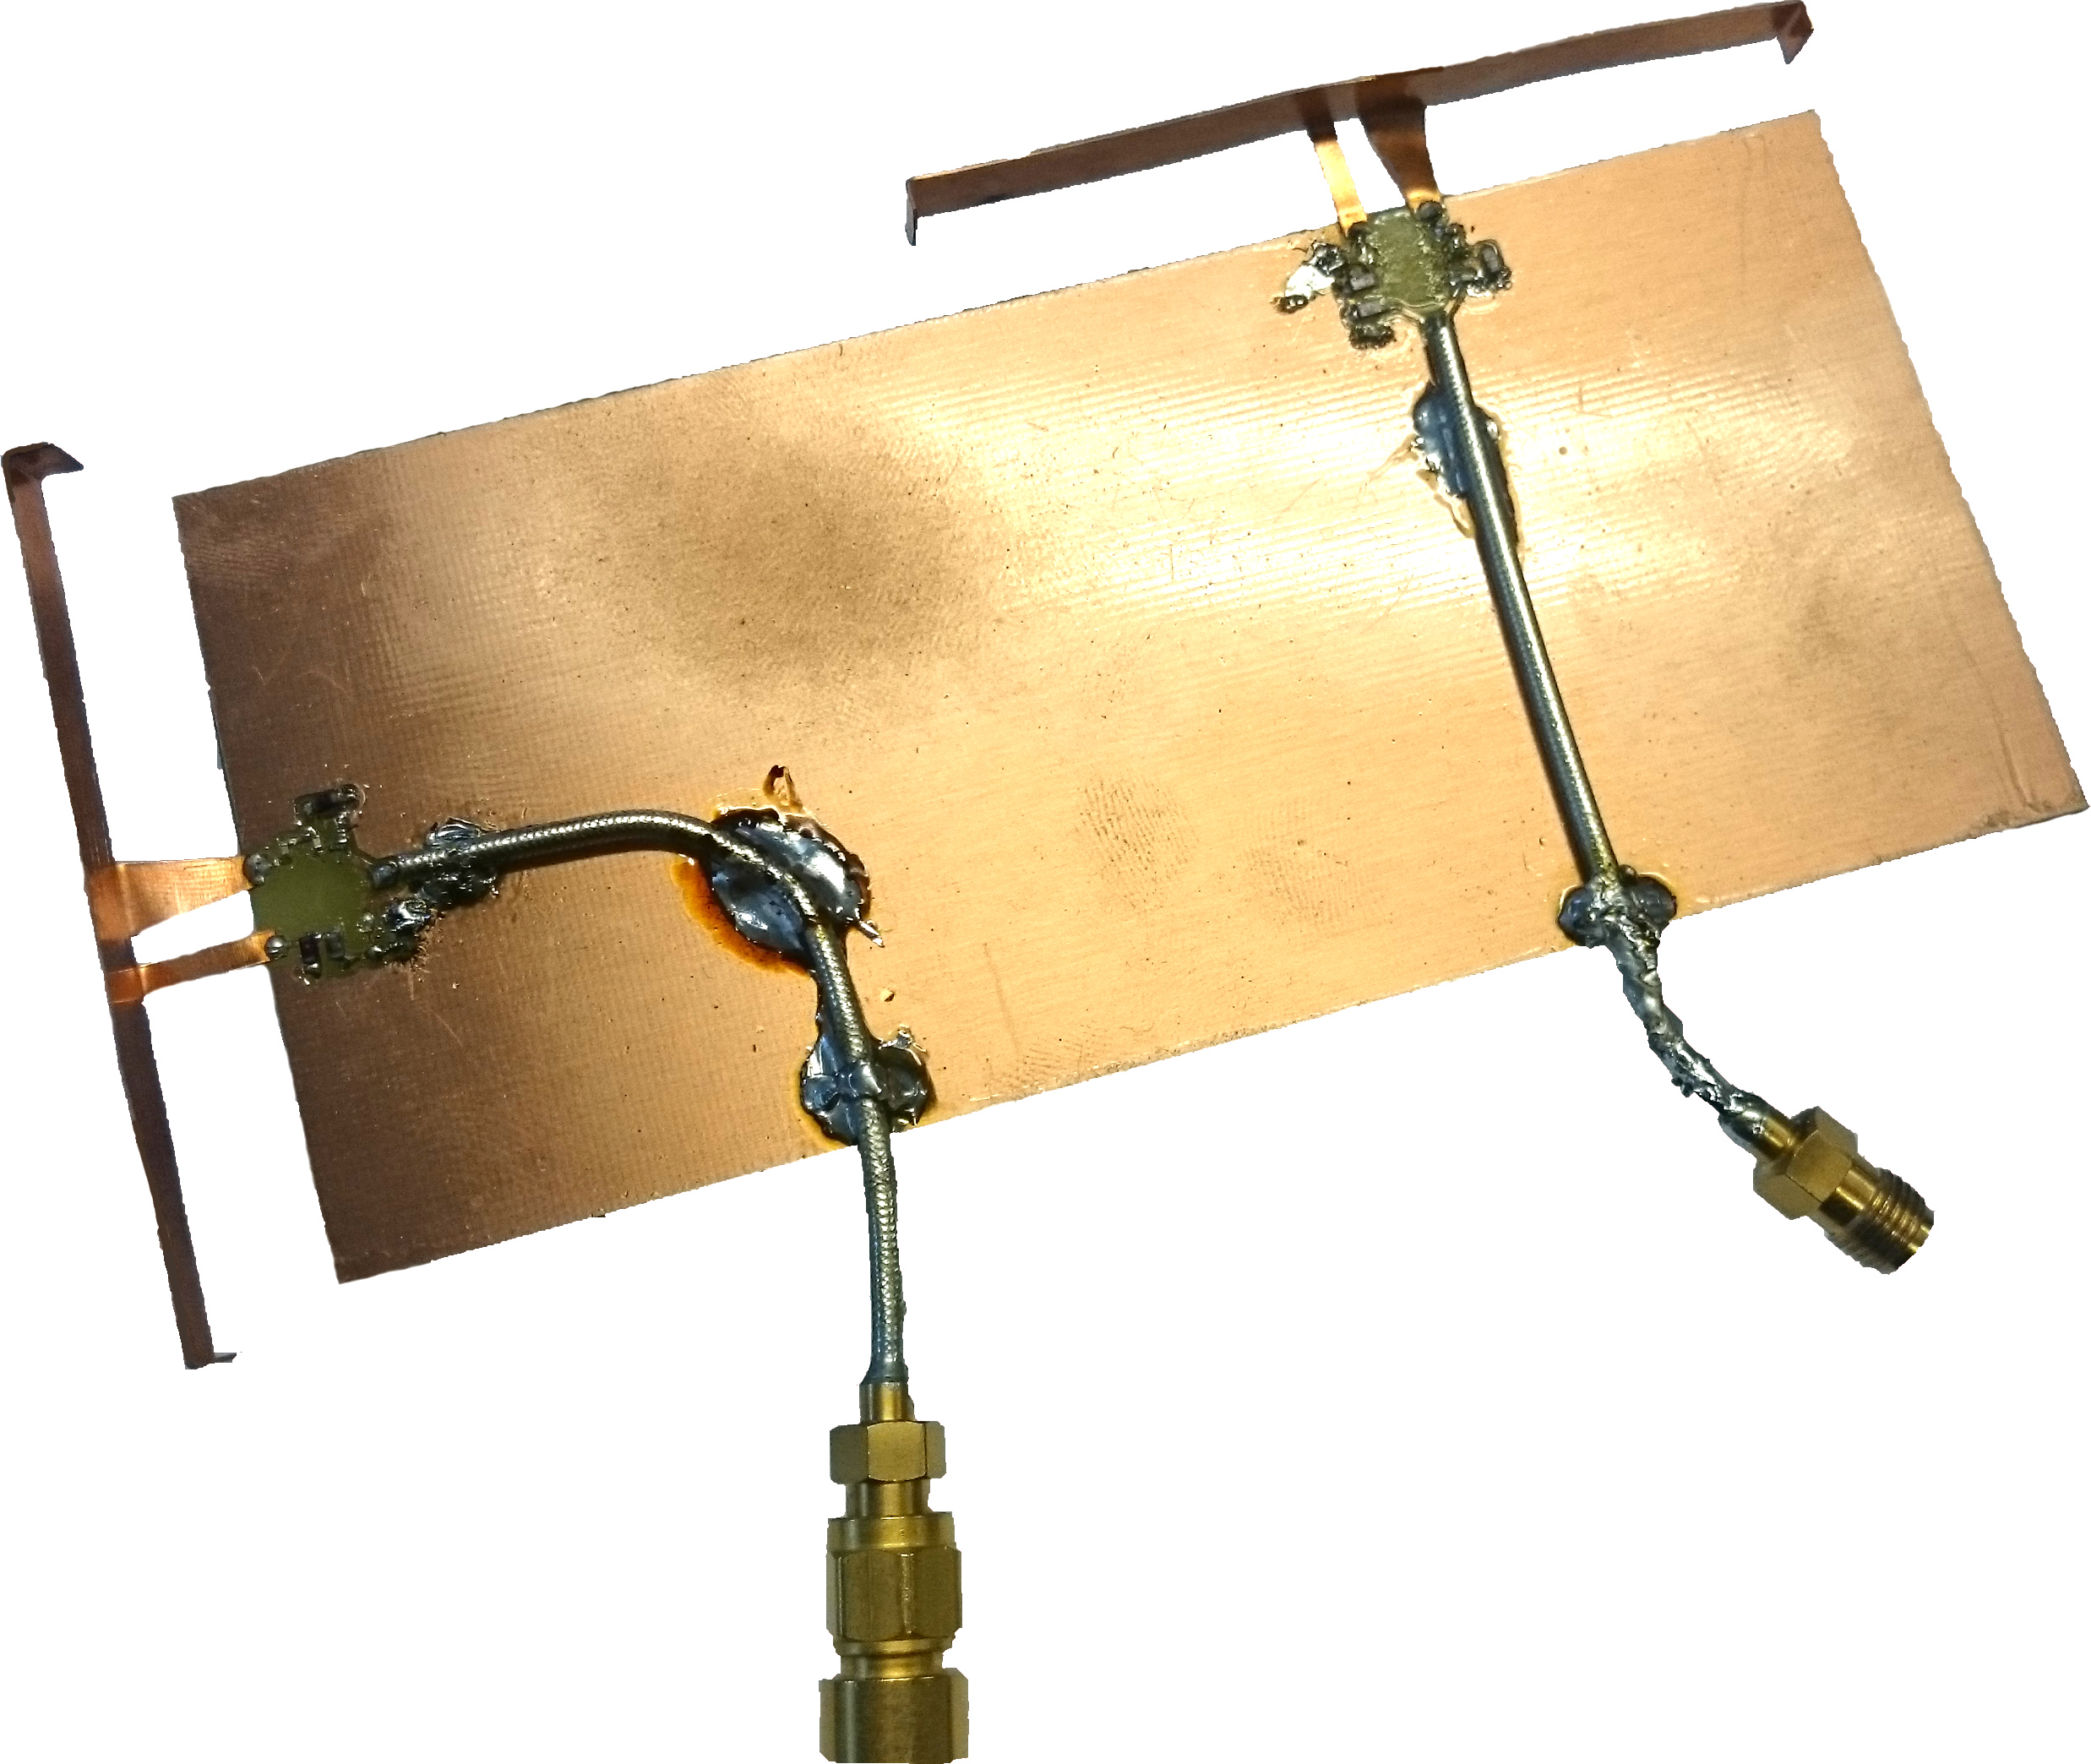
\includegraphics[scale=0.1]{img/tech_sol/nonresonant/prototype/3d_figure.jpg}
        \caption{Non-resonant antenna prototype.}
        \label{fig:nonresonant_proto}
    \end{subfigure}
    \hfill
    \begin{subfigure}[b]{0.49\linewidth}
        \centering
        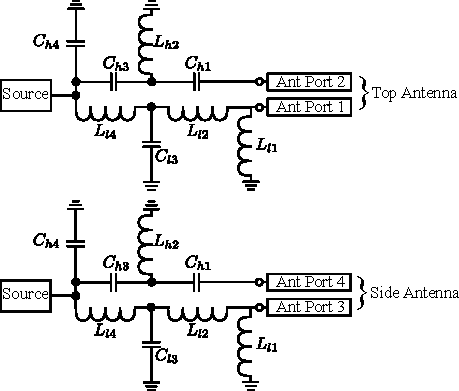
\includegraphics{img/tech_sol/nonresonant/schematic_tuning}\\[0cm]
        \caption{Tuning/matching circuit.}
        \label{fig:ant3schematic}
    \end{subfigure}
    \caption{Picture and tuning circuit for the prototype antenna.  The antennas are built on FR-4 board using \SI{35}{\micro\meter} copper. There is a matching circuit as shown for each of the four feeds.}
    \label{fig:ant3techschem_proto}
\end{figure}


\subsection{Measurement and Simulation Comparison}
The simulated and measured S-parameter and total efficiency is shown in Figure \ref{fig:nonresonant_proto_matching}. The results are done with the tunable capacitor at \SI{0.3}{pF}. Furthermore some adjustments were done to the component values, the current values can be seen in Table \ref{fig:ant3schematic_proto}. 
 \begin{figure}[htbp]
    \centering
    \begin{subfigure}{0.49\linewidth}
        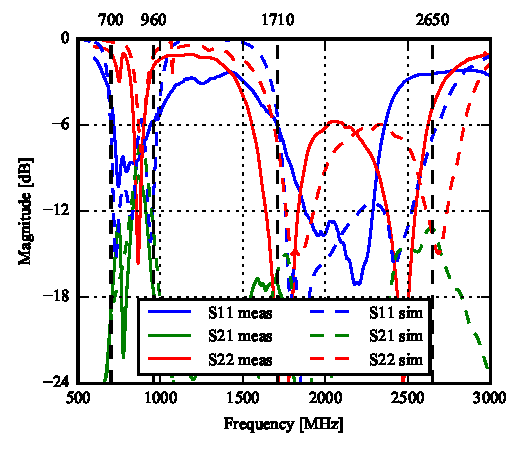
\includegraphics{img/tech_sol/nonresonant/prototype/sparams.pdf}
        \caption{S-parameters.}
    \end{subfigure}
    \hfill
    \begin{subfigure}{0.49\linewidth}
    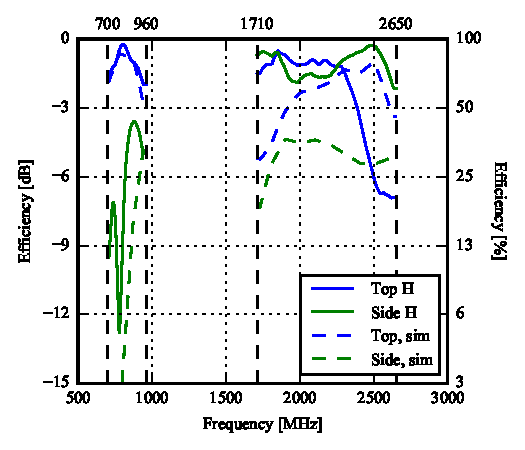
\includegraphics{img/tech_sol/nonresonant/prototype/eff_comp.pdf}
        \caption{Total efficiency.}
    \end{subfigure}
    \caption{S-parameters and total efficiency of the nonresonant antenna prototype with the component values from Figure~\ref{fig:nonresonant_proto_matching}.}
    \label{fig:nonresonant_proto_sparam_eff}
\end{figure}

   \begin{table}
      \centering
      \begin{tabular}{|l|l|r|r|r|}
        \hline
        Antenna & Band & Start [MHz] & Stop [MHz] & Bandwidth [MHz] \\
        \hline
        Top     & Low  & 700        & 960       & 260 \\
        Side    & Low  & 830         & 910        & 80 \\
        \hline
        Top     & High & 1710        & 2350       & 640 \\
        Side    & High & 1550        & 2645       & 1095 \\
        \hline
      \end{tabular}
      \caption{Maximum bandwidth obtained in the low and high band for the top and the side antenna, respectively.}
      \label{tab:bw_sol3_proto}
    \end{table}

\begin{table}
  \centering
        \begin{tabular}{|l|l|l|l|l|l|l|l|l|}
            \hline
                         & $L_{l1}$       & $L_{l2}$        & $C_{l3}$      & $L_{l4}$       & $C_{h1}$       & $L_{h2}$      & $C_{h3}$      & $C_{h4}$    \\
            \hline
            Top antenna  & \SI{10}{nH}  & \SI{15}{nH}  & \SI{3}{pF} & \SI{5.6}{nH} & \SI{1.2}{pF} & \SI{7.5}{nH} & \SI{3}{pF} & \SI{0.1}{pF} \\
            Side antenna & \SI{10}{nH}  & \SI{16}{nH}  & \SI{6.8}{pF} & \SI{4.3}{nH} & \SI{0.7}{pF} & \SI{5.1}{nH} & \SI{2.2}{pF} & \SI{1.2}{pF} \\
            \hline
        \end{tabular}
        \caption{Component values}
        \label{fig:ant3schematic_proto}
\end{table}

\FloatBarrier
\section{Capacitor sweep}
\begin{figure}[htbp]
    \centering
    \begin{subfigure}{0.49\linewidth}
        \centering
        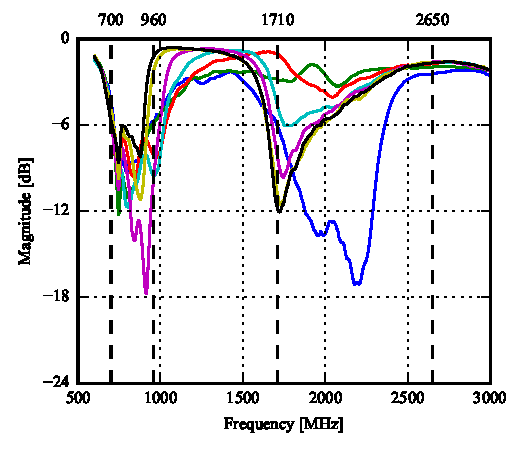
\includegraphics{img/tech_sol/nonresonant/prototype/s11_csh1.pdf}
        \caption{$S_{11}$, sweeping the top antenna and fixing the side antenna.}
    \end{subfigure}
    \hfill
    \begin{subfigure}{0.49\linewidth}
        \centering
        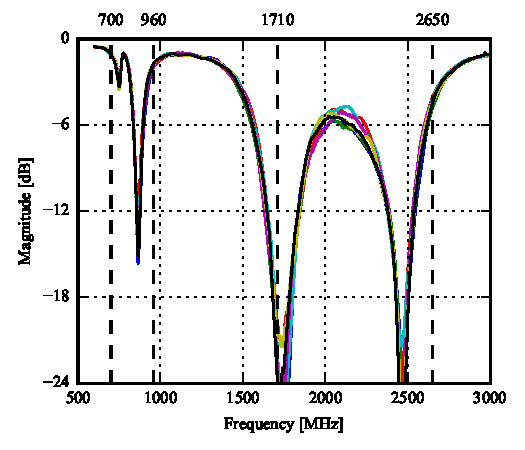
\includegraphics{img/tech_sol/nonresonant/prototype/s22_csh1.pdf}
        \caption{$S_{22}$, sweeping the side antenna and fixing the top antenna.}
    \end{subfigure}
    \\
    \begin{subfigure}{0.49\linewidth}
        \centering
        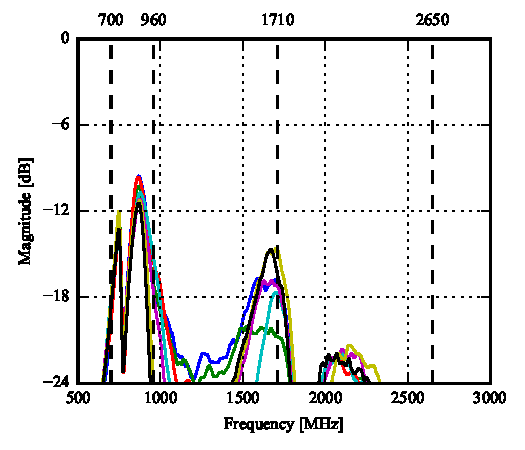
\includegraphics{img/tech_sol/nonresonant/prototype/s21_csh1.pdf}
        \caption{$S_{21}$, sweeping the top antenna and fixing the side antenna.}
    \end{subfigure}
    \hfill
    \begin{subfigure}{0.49\linewidth}
        \centering
        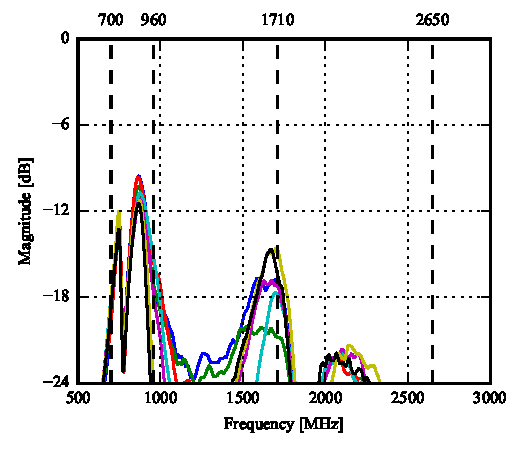
\includegraphics{img/tech_sol/nonresonant/prototype/s12_csh1.pdf}
        \caption{$S_{21}$, sweeping the side antenna and fixing the top antenna.}
    \end{subfigure}
    \caption{Non-resonant antenna. S-parameters for different shunt-capacitor values.}
    \label{fig:nonresonant_proto_sweep_sparams}
\end{figure}

\begin{figure}[htbp]
    \centering
    \begin{subfigure}{0.49\linewidth}
        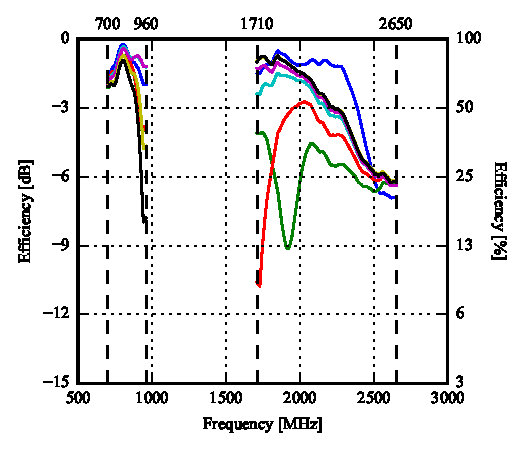
\includegraphics{img/tech_sol/nonresonant/prototype/efficiency_top.pdf}
        \caption{Top antenna, sweeping the top antenna and fixing the side antenna.}
    \end{subfigure}
    \hfill
    \begin{subfigure}{0.49\linewidth}
        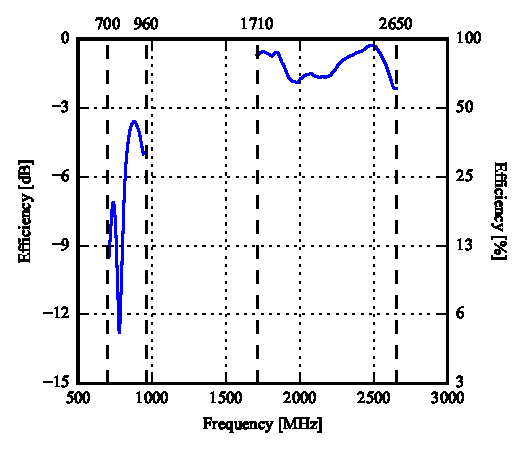
\includegraphics{img/tech_sol/nonresonant/prototype/efficiency_side.pdf}
        \caption{Side antenna, sweeping the side antenna and fixing the top antenna.}
    \end{subfigure}
    \caption{Total efficiency for each of the antennas when sweeping the shunt-capacitor values.}
    \label{fig:nonresonant_proto_sweep_efficiency}
\end{figure}